\section{Work Allocation (ps)}

In order to ensure that the group functions effectively, the work must be allocated to the group members and the group ressources must be managed. The group members analysed the specification of the project well to best suit the tasks to the member's skills. The work will be allocated on a regular basis. The following factors have been considered thoroughly before assigning tasks to any team members:

\begin{itemize}
\item	Availability of each member. 

\item	The number of members that can work on a single task.

\item  The deadline of the task.

\item	The skills required for the task
\end{itemize}


\subsection*{Planned Work Allocation}
\label{sec:work_plan}

It is very essential that the other obligations of the group members are taken consideration during work allocation. 
The group members will work effectively if they are assigned work they are interested in with well clarified roles. This can be determined using a skills audit.
The skills audit highlights the skills and knowledge the group members possess prior to the task. 
Each task has been assigned a task leader who will work with their co-workers when problems are encountered during their task.
In order to avoid tasks overrunning, the tasks have been set earlier deadlines so that there is spare time to handle unexpected problems. 

The results of the skill audit are:

\begin{itemize}
\item Andy: Power, PCB, Control, MATLAB
\item Mitch: Image Processing, MATLAB, ASM, Report Writing
\item John: MATLAB, Image Processing, Control, Radio Transmission
\item Peak: Digital Control, Display, MATLAB, Information Theory
\item Michael: Programming, $\mu$Processors, Interfaces
\end{itemize}

The dependencies of the tasks are also important to consider. 
This may cause problems when tasks with many dependencies get stuck and cause many tasks to delay. 
This can be solved by well partitioning the tasks so that there is always a task available when others can't be completed. 

The required number of people per task limits the task allocation. The customer has only provided a single UAV and only one camera should been purchased, so only one person can work on each device at a time. This is mitigated by having a laboratory space where the UAV will be placed at all times so that any team member can access it. To manage the limited resources, the only time that the individual can access the UAV is when he wants to test the system. 

It is important to clarify the tasks and ensure that all tasks are properly assigned. 
Figure\ref{task allocation} shows how the tasks are allocated between each member of the group. 
The blue box between members are shared tasks. 
If the blue box stand on its own it means only one person is assigned to that task.

\begin{figure}[H]
\begin{center}
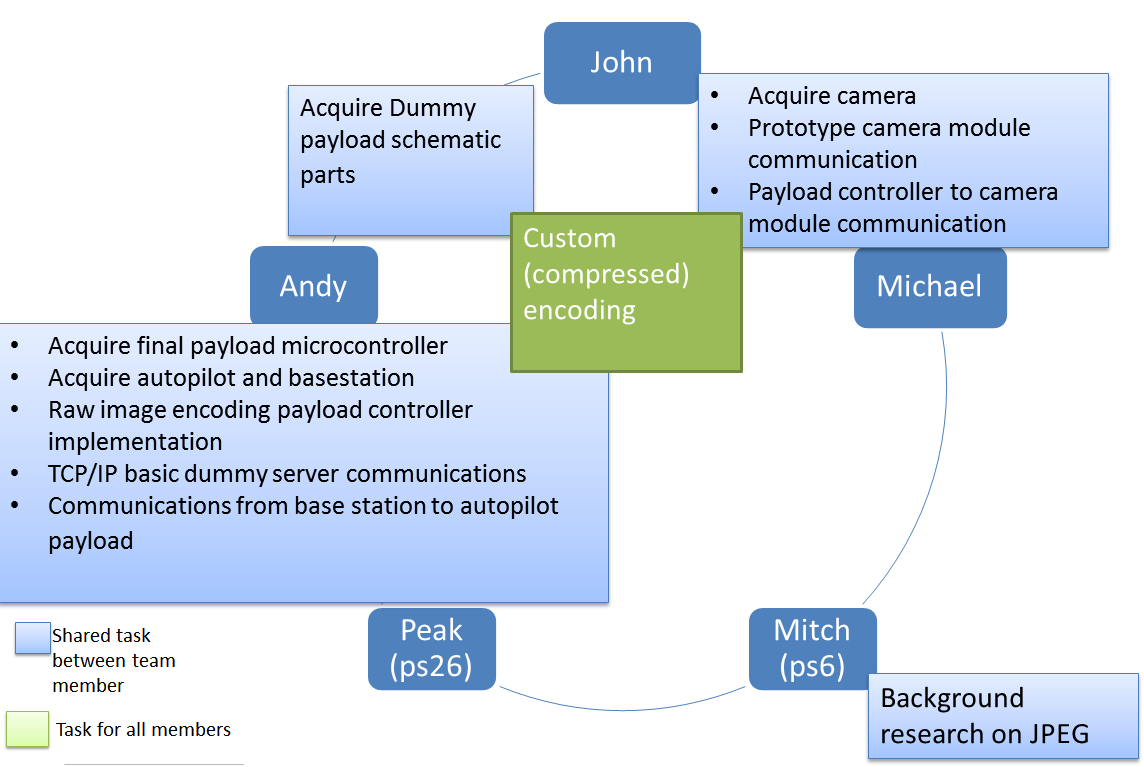
\includegraphics[width=1.0\textwidth]{figures/initial_task_allocation.png} 
\end{center}
\caption{Initial task allocation of the project\label{task allocation}}
\end{figure}

\subsubsection{Schedule - (jc)}
Considerable thought was also given to the scheduling of the tasks, an initial Gantt chart was drawn up
at the beginning of the project (see appendix \ref{appendix:gantt}) with a breakdown of the tasks as we
imagined them at the start of the project.

During our regular meetings this Gantt chart was used as a gauge for our progress and was amended when
needed (i.e. our initial timing turned out to be slightly optimistic).
